% Author: Zdeněk Lapeš <lapes.zdenek@gmail.com> (xlapes02)


\documentclass[a4paper, 11pt]{article}


\usepackage[czech]{babel}
\usepackage[utf8]{inputenc}
\usepackage[left=2cm, top=3cm, text={17cm, 24cm}]{geometry}
\usepackage{xcolor}
\usepackage{times}
\usepackage{graphicx}
\usepackage{float}

\usepackage[unicode]{hyperref}
\graphicspath{ {images/} }
\hypersetup{
    colorlinks = true,
    hypertexnames = false,
    citecolor = red
}
\usepackage{listings}

\definecolor{mGreen}{rgb}{0,0.6,0}
\definecolor{mGray}{rgb}{0.5,0.5,0.5}
\definecolor{mPurple}{rgb}{0.58,0,0.82}
\definecolor{backgroundColour}{rgb}{0.95,0.95,0.92}

\lstdefinestyle{CStyle}{
    backgroundcolor=\color{backgroundColour},
    commentstyle=\color{mGreen},
    keywordstyle=\color{magenta},
    numberstyle=\tiny\color{mGray},
    stringstyle=\color{mPurple},
    basicstyle=\footnotesize,
    breakatwhitespace=false,
    breaklines=true,
    captionpos=b,
    keepspaces=true,
    numbers=left,
    numbersep=5pt,
    showspaces=false,
    showstringspaces=false,
    showtabs=false,
    tabsize=2,
    language=C
}
\lstset{basicstyle=\ttfamily,
    showstringspaces=false,
    commentstyle=\color{red},
    keywordstyle=\color{blue}
}




\begin{document}
    %%%%%%%%%%%%%%%%%%%%%%%%%%%%%%%% Titulní stránka %%%%%%%%%%%%%%%%%%%%%%%%%%%
    \begin{titlepage}
        \begin{center}
            
\includegraphics[width=0.77\linewidth]{FIT_logo} \\

            \vspace{\stretch{0.382}}

            \Huge{Projektová dokumentace} \\
            \LARGE{\textbf{
                Tunelování datových přenosů přes DNS dotazy
            }} \\
            \Large{Síťové aplikace a~správa sítí}

            \vspace{\stretch{0.618}}
        \end{center}

        {\Large
        \today
        \hfill
        Zdeněk Lapeš (xlapes02)
        }
    \end{titlepage}


    %%%%%%%%%%%%%%%%%%%%%%%%%%%%%%%% Obsah %%%%%%%%%%%%%%%%%%%%%%%%%%%%%%%%%%%%%
    \pagenumbering{roman}
    \setcounter{page}{1}
    \tableofcontents
    \clearpage
    \pagenumbering{arabic}
    \setcounter{page}{1}


    %%%%%%%%%%%%%%%%%%%%%%%%%%%%%%%% Content %%%%%%%%%%%%%%%%%%%%%%%%%%%%%%%%%%%%%%
    \section{Úvod}
\label{sec:uvod}
Cílem projektu bylo vytvořit aplikaci pro tunelování datových přenosů pomocí
DNS dotazů v~jazyce C\@. Aplikace by měla umožnit přenášet data mezi klientem
a serverem.
Klient posílá DNS dotazy se zakodovanými daty do qname na DNS server,
který dotazy zpracovavá, ukláda do souboru a~posílá odpověď klientovi.
Aplikace by měla umožnit přenášet data ze souboru a standardního vstupu.

Oba programy (\texttt{dns\_sender} a \texttt{dns\_receiver}) je možné
ovládat přes vstupní argumenty programu, viz\ref{sec:usage}.

%%%%%%%%%%%%%%%%%%%%%%%%%%%%%%%% Popis DNS Tunelovaní %%%%%%%%%%%%%%%%%%%%%


\section{Popis mechanismu pro tunelování datových přenosů prostřednictvím DNS dotazů}
\label{sec:popis-mechanismu-pro-tunelovani-datovych-prenosu-prostrednictvim-dns-dotazu}

Domain name system, DNS je protokol překládající url adresu na ip adresu.
DNS dotaz je zpráva, která se posílá na DNS server, který odpoví na dotaz.
DNS dotaz je složen z hlavičky a těla dotazu\cite{dnsPacket}.

Tunelování pomocí DNS dotazu využívají utočníci, kteří
mají na svém serveru nainstalovaný malware.
Klientův dotaz je směrován na utočníkům server, kterému to umožní
nainstalovat malware na klientovi a provádět další akce.

    \section{Popis návrhu a implementace klientské a serverové aplikace}
\label{sec:popis-navrhu-a-implementace-klientske-a-serverove-aplikace}
Adresářová struktura:

Adresářová struktura je rozdělena do 3 adresářů.

\begin{itemize}
    \item \texttt{sender} \- obsahuje zdrojové soubory pro klienta
    \item \texttt{receiver} \- obsahuje zdrojové soboury pro serveru
    \item \texttt{common} \- obsahuje zdrojové soubory, které jsou využívány\\
    obema programy \texttt{dns\_sender} a \texttt{dns\_receiver}
    \item \texttt{middleman} \- obsahuje kód pro otestování ztráty \\
    packetu (Pouze jako ukázka otestování, při běžném běhu aplikaci se nepoužívá).\\
    Makro \texttt{TEST\_LOSS\_PACKET} nacházející se v \texttt{./commmon/dns\_helper.h} zapne middlemana.
\end{itemize}

Oba programy jsou řízeny stavovým automatem, který rozlišuje stav
na základě typu paketu a podle
něho provadí další specifické kroky pro vytvaření dotazů a odpovědí.


%%%%%%%%%%%%%%%%%%%%%%%%%%%%%%%% Klient %%%%%%%%%%%%%%%%%%%%%%%%%%%%%%%%

\subsection{Klient \- dns\_sender}
Na začátku programu jsou alokovány a inicializovány celkem 3 struktury.
\begin{itemize}
    \item \texttt{program\_t} \- obsahuje všechny promměnné programu
    \item \texttt{dns\_datagram\_t} \- obsahuje všechny promměnné datagramu
    \item \texttt{args\_t} \- obsahuje všechny vstupní promměnné programu
\end{itemize}

\subsubsection{Parsovaní argumentu} \label{sec:parsovani-argumentu-k}
Vstupní argumenty klienta jsou parsovaný pomocí vlastní algoritmické
implementace, kvůli několika druhům argumentů
(povinné poziční, povinné nepoziční, nepovinné poziční).

Parsování zajišťuje funkce \texttt{void set\_args\_sender(program\_t *program)} \\
v souboru \texttt{common/argument\_parser.c}.

\subsubsection{Vytváření paketu a čtení ze souboru} \label{sec:vytvareni-paketu-k}

Paket je vytvářen podle aktuálního typu packetu, kterých je celkem 5 druhů:

\paragraph{START}
Informační paket, následující paket bude obsahovat název cílového souboru.
Při tomto typu paketu se nastaví \texttt{program\->dgram\->packet\_type} na \texttt{FILENAME}.

V qname DNS dotazu je pouze \texttt{ZAKODOVANY\_STRING\_"START".BASEHOST}.

\paragraph{FILENAME}
Paket obsahující název cílového souboru.

Délka cílového souboru je omezena na 1024 znaku.

Soubor je postupně rozparsován a zakódován
do více paketů v případě, že není možné název souboru
zakódovat do jednoho qname DNS dotazu,
jehož maximální povolená délka je 255 znaků\cite{dnsPacketInfo}.

V qname DNS dotazu je \texttt{ZAKODOVANY\_FILENAME.BASEHOST}.

\paragraph{DATA}
Informační paket, že následující paket bude obsahovat data souboru.

V qname DNS dotazu je pouze \texttt{ZAKODOVANY\_STRING\_"DATA".BASEHOST}.

\paragraph{SENDING}
Paket obsahující data souboru/stdin.

Obsah souboru je postupně čten, rozparsován a zakodován do qname DNS dotazu.
Soubor se čte postupne podle možné délky dat pro
zakodování do qname, kterou počítám makrem nacházejícího se v souboru \\
\texttt{common/dns\_helper.c}: \\
\texttt{\#define BASE32\_LENGTH\_DECODE(src\_size) (ceil((src\_size) / 1.6))}. \\
Makro jako vstup bere maxímální délku po zakódování a vrácí délku před zakodováním.
V případě, že není možné data zakódovat do jednoho qname DNS dotazu,
tak je soubor rozdělen na více paketů.

V qname DNS dotazu je \texttt{ZAKODOVANY\_DATA.BASEHOST}.

\paragraph{END}
Informační koncový paket, že všechna data byla přenesena.

V qname DNS dotazu je \texttt{ZAKODOVANY\_STRING\_"END".BASEHOST}.

\subsubsection{Odeslani dotazu} \label{sec:odeslani-dotazu-k}
Dotaz je odeslán okamžitě při každém vytvoření paketu viz\ref{sec:vytvareni-paketu-k}.
Pro zakódování dat se používá funkce: \\
\texttt{int base32\_encode(const uint8\_t *data, int length, \\
uint8\_t *result, int bufSize)}\cite{encodingData}.

\subsubsection{Prijimani odpovedi}\label{sec:prijimani-odpovedi-k}
Klient očekává odpověď, pokud nedorazí do 5 sekund, tak klient odešle paket znova.
To je řešeno pomocí funkce následujícího volání funkce:
\texttt{setsockopt(dgram\->network\_info.socket\_fd, \\
    SOL\_SOCKET, SO\_RCVTIMEO, \&timeout, sizeof(timeout))},\\
které se provádí v souboru \texttt{common/initialization.c}.


%%%%%%%%%%%%%%%%%%%%%%%%%%%%%%%% Server %%%%%%%%%%%%%%%%%%%%%%%%%%%%%%%%

\subsection{Server \- dns\_receiver}

Na začátku programu jsou alokovány celkem 3 struktury.

\begin{itemize}
    \item \texttt{program\_t} \- obsahuje všechny promměnné programu
    \item \texttt{dns\_datagram\_t} \- obsahuje všechny promměnné datagramu
    \item \texttt{args\_t} \- obsahuje všechny vstupní promměnné programu
\end{itemize}

\subsubsection{Parsování argumentů} \label{sec:parsovani-argumentu-s}

Argumenty serveru jsou parsovány pomocí knihovní funkce \texttt{getopt}, \\
kvůli vypisování nápovědy. Všechny ostatní argumenty jsou poziční a povinné,
což zjednodušuje parsování vstupních argumentů programu.

Parsování zajišťuje funkce \texttt{void set\_args\_receiver(program\_t *program)} \\
v souboru \texttt{common/argument\_parser.c}.

\subsubsection{Parsování paketu a ukládání dat do souboru} \label{sec:vytvareni-paketu-s}
Paket je parsovaným podle aktualního typu packetu, kterých je serveru
rozlišujeme celkem 8 druhů:

\paragraph{START}
Informační paket, následující paket bude obsahovat název cílového souboru.

Při tomto typu paketu se nastaví \texttt{program\->dgram\->packet\_type} \\
na \texttt{FILENAME}.

\paragraph{FILENAME}
Paket obsahující název cílového souboru.

Délka cílového souboru je omezena na 1024 znaků.

Cílový soubor je parsován v nekonecné smyčce z qname DNS dotazu\\
a uložen do proměnné \texttt{program\->args\->filename}, dokud nepříjde\\
další informační paket s daty \texttt{DATA}.

\paragraph{DATA}
Informační paket, že následující paket bude obsahovat data souboru.

Při tomto typu paketu se nastaví \texttt{program\->dgram\->packet\_type} na \texttt{SENDING}.

\paragraph{SENDING}
Paket obsahující data souboru/stdin.

Data jsou z qname DNS dotazu parsována, dekódována a
zapisována do souboru v nekonečné smyčce, dokud nepřijde další
informační paket s daty \texttt{END}.

\paragraph{END}
Informační koncový paket, že data byla přenesena.

Při tomto typu paketu se nastaví \texttt{program\->dgram\->packet\_type} na \texttt{WAITING\_NEXT\_FILE}.

\paragraph{WAITING\_NEXT\_FILE}
Čeka se na prenos dalšího souboru.

\paragraph{RESEND\_OR\_BADBASEHOST\_\_AFTER\_FILENAME}
Chyba v base host, nebo je paket přenášen znovu, protože někde nastala chyba.
Do tohodle stavu se přejde, pokud aktuální stav je \texttt{FILENAME}.

\paragraph{RESEND\_OR\_BADBASEHOST\_\_AFTER\_SENDING}
Chyba v base host, nebo je paket přenášen znovu, protože někde nastala chyba.
Do tohodle stavu se přejde, pokud aktuální stav je \texttt{SENDING}.

\subsubsection{Příjem dotazu} \label{sec:odeslani-dotazu-s}
Při příjmu dat se pro dekódování používá funkce
\texttt{ int base32\_decode(const uint8\_t *encoded, uint8\_t *result, int bufSize) }\cite{encodingData}.

\subsubsection{Odeslani odpovedi}\label{sec:prijimani-odpovedi-s}
Po úspěšném zápisu dat do souboru se odešle odpověď na dotaz.
K DNS dotazu se přidá answer a paket se odešle zpět.

    \section{Testovani klientské a serverové aplikace}\label{sec:testovani}
Testování probíhalo ručně za použití aplikace Wireshark a funkcí
ze souboru \texttt{middleman/middleman.c} a \texttt{middleman/middleman.h}
(testování spolehlivého doručení).

Testovací/Debugovací makra:
\begin{itemize}
    \item \texttt{DEBUG} \- Zapne nebo vypne debugovací výpisy
    \item \texttt{TEST\_LOSS\_PACKET} \- Zapne nebo vypne zdrojový kód
    \texttt{middleman/middleman.c}, který náhodně zahazuje pakety
    a tím se testuje případná ztráta paketu.
    \item \texttt{EVENT} \- Zapne nebo vypne funkce z poskytnutého API k projektu.
\end{itemize}

\paragraph{Ztrata paketu od klienta}
Ztráta paketu je řešena pomocí timeoutu na straně klienta, který pošle
paket znovu pokud nedorazí odpověď od severu po dobu 5 sekund.

\paragraph{Ztrata paketu od serveru}
Pokud na server dorazí paket se stejným id jako paket měl
paket předchozí, server
paket nijak nezpracuje a odešle stejnou odpoveď jako předchozí.

\begin{figure}[H]
    \centering
    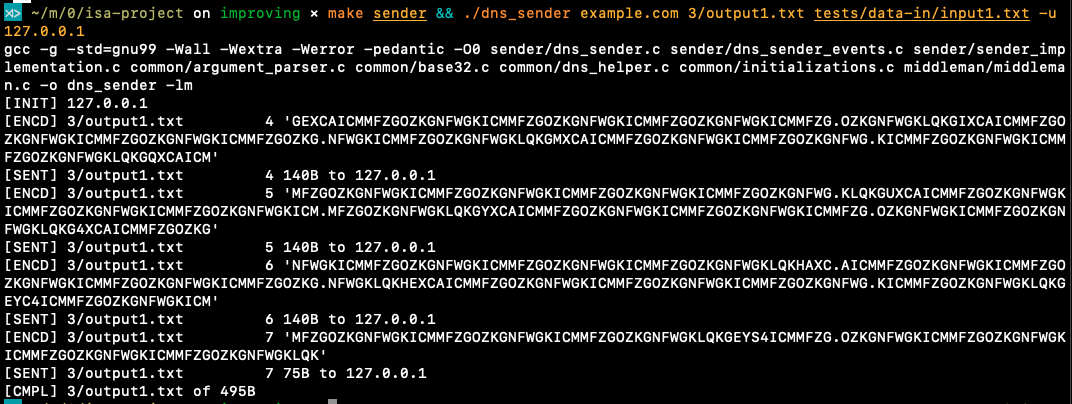
\includegraphics[width=0.77\textwidth]{sender}
    \caption{Ukázka komunikace od klienta}
    \label{fig:a1}
\end{figure}

\begin{figure}[H]
    \centering
    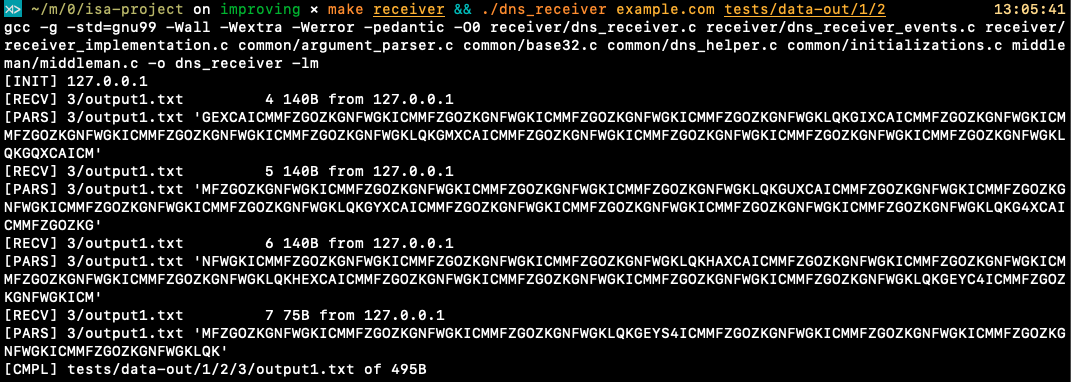
\includegraphics[width=0.77\linewidth]{receiver}
    \caption{Ukázka komunikace od serveru}
    \label{fig:a2}
\end{figure}

\begin{figure}[H]
    \centering
    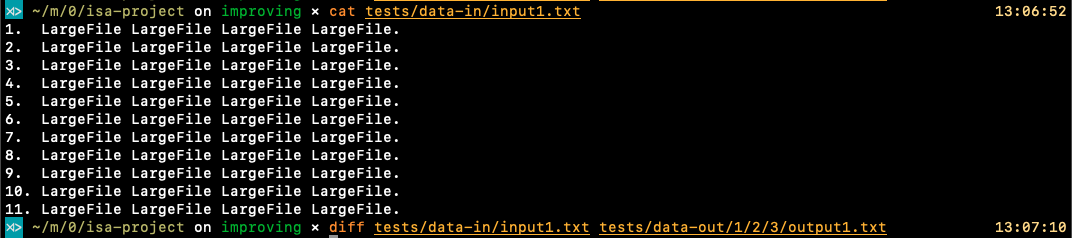
\includegraphics[width=0.77\linewidth]{diff}
    \caption{Ukázka otestovani preneseneho souboru}
    \label{fig:a4}
\end{figure}

\begin{figure}[H]
    \centering
    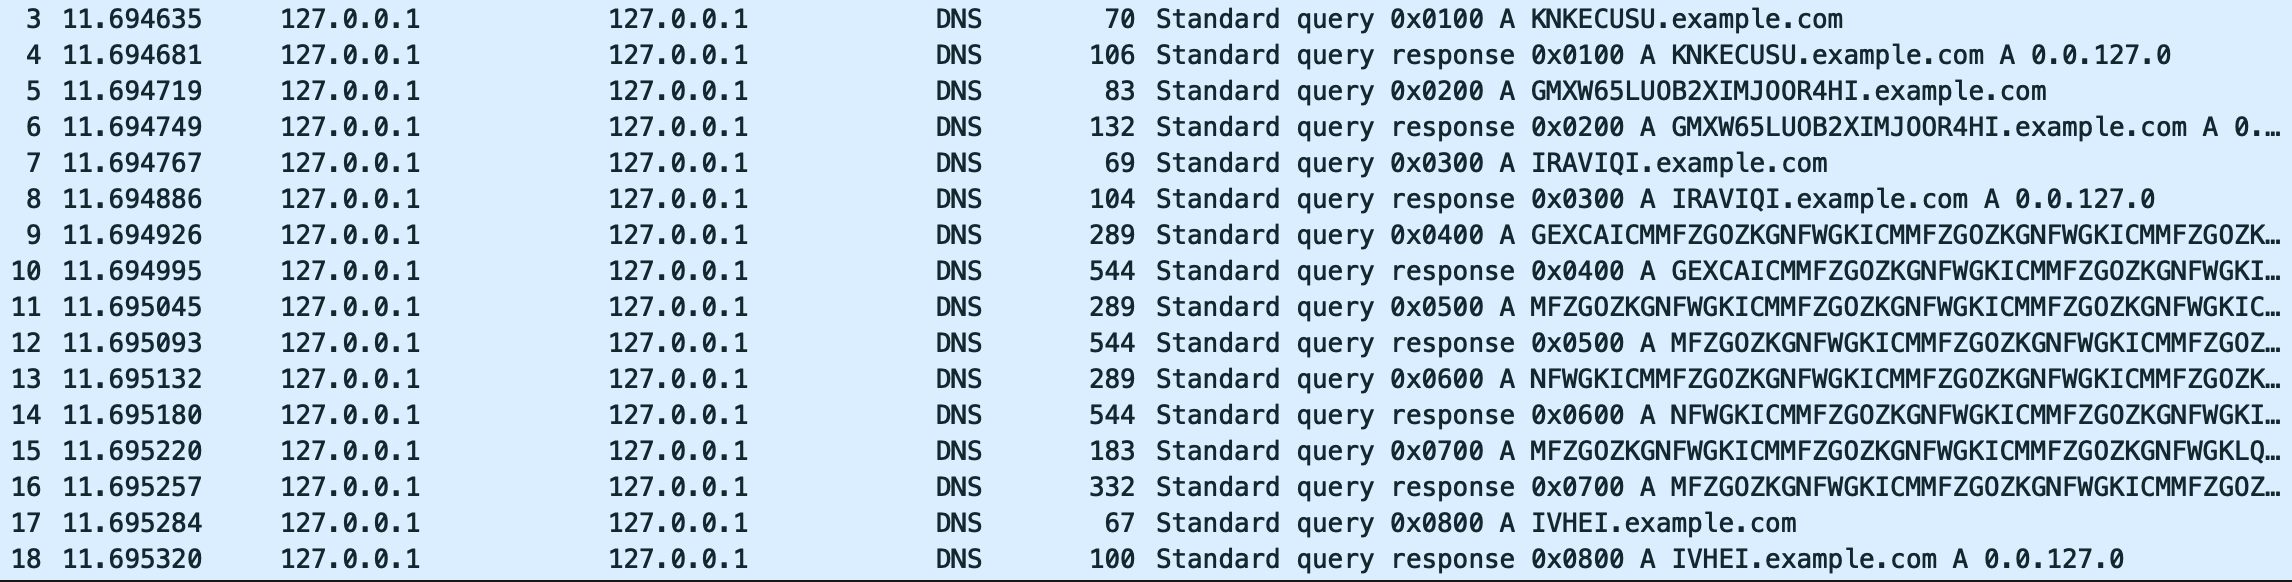
\includegraphics[width=0.77\linewidth]{wireshark}
    \caption{Ukázka komunikace v aplikaci Wireshark}
    \label{fig:a5}
\end{figure}

    %%%%%%%%%%%%%%%%%%%%%%%%%%%%%%%%%%%%%%%
%%%%%%%%%%%%%%%%%%%%%%%%%%%%%%%% Návod na použití %%%%%%%%%%%%%%%%%%%%%%%%%%
\section{Návod na použití} \label{sec:usage}

\subsection{Překlad}\label{section:compilation}

Překlad je prováděn pomocí aplikace \texttt{GNU Make}.
Soubor s definicí překladu se nacházi v~souboru \texttt{Makefile}.\\
Podporované argumenty pro přikaz \texttt{make} jsou:

\begin{itemize}
    \item \texttt{make} Prelozi obe aplikace
    \item \texttt{make all} Přeloží obě aplikace
    \item \texttt{make sender} Přeloží pouze aplikaci \texttt{dns\_sender}
    \item \texttt{make receiver} Přeloží pouze aplikaci \texttt{dns\_receiver}
    \item \texttt{make pack} Zabalí projekt
\end{itemize}

Obě aplikace se po překladu nachází v~kořenovém adresáři projektu.

\subsection{Spouštění programu \texttt{dns\_sender}}

\texttt{dns\_sender [-u UPSTREAM\_DNS\_IP] {BASE\_HOST} {DST\_FILEPATH} [SRC\_FILEPATH]}

\textit{Přepínače:}

\begin{itemize}
    \item \texttt{-u <UPSTREAM\_DNS\_IP>} Slouží k vynucení vzdáleného DNS serveru
\end{itemize}

\textit{Poziční parametry:}

\begin{itemize}
    \item \texttt{BASE\_HOST} Slouží k nastavení bázové domény všech přenosů
    \item \texttt{DST\_FILEPATH} Cesta pod kterou se data uloží na serveru
    \item \texttt{SRC\_FILEPATH} Cesta k souboru který bude odesílán, pokud není specifikováno pak program čte data ze STDIN
\end{itemize}

Povinné parametry jsou \texttt{BASE\_HOST}, \texttt{DST\_FILEPATH}.

Při chybně zadaných parametrech se vypíše napověda programu.
Nápovědu je možné si vypsat také \\
příkazem \texttt{./dns\_sender -h}.

\subsection{Spouštění programu \texttt{dns\_receiver}}

\texttt{dns\_receiver {BASE\_HOST} {DST\_DIRPATH}}

\textit{Poziční parametry:}
\begin{itemize}
    \item \texttt{BASE\_HOST} Slouží k nastavení bázové domény všech přenosů
    \item \texttt{DST\_DIRPATH} Cesta pod kterou se budou všechny příchozí data/soubory ukládat
\end{itemize}

Povinné parametry jsou \texttt{BASE\_HOST}, \texttt{DST\_DIRPATH}.

Při chybně zadaných parametrech se vypíše napověda programu.
Nápovědu si je možné vypsat také \\
příkazem \texttt{./dns\_receiver -h}.

    %%%%%%%%%%%%%%%%%%%%%%%%%%%%%%%% Závěr %%%%%%%%%%%%%%%%%%%%%%%%%%%%%%%%%%%%%
\section{Závěr}

Naimplementoval jsem kompletní a funkční aplikace, podle specifikace projektu.

Projekt se mi nejevil jako obtížná, ale i tak jsem se v některých
částech implemenatce strávil více času než sem očekával.

Vypracování projektu mi pomohlo získat dobrou představu o DNS protokolu a
o jeho implementaci. Dobu na vypracování projektu odhaduji na cca 30-40 hodin.

Celkově jsem spokojen s výsledkem.


    %%%%%%%%%%%%%%%%%%%%%%%%%%%%%%%% Citace %%%%%%%%%%%%%%%%%%%%%%%%%%%%%%%%%%%%
    \clearpage
    \bibliographystyle{bib/czechiso}
    \renewcommand{\refname}{Literatura}\label{sec:literatura}
    \bibliography{manual}

\end{document}
